%!TEX root = main.tex
\setcounter{chapter}{3}
\setcounter{section}{9}
\setcounter{theorem}{0}
\setcounter{equation}{0}

\lectureheader{161}{Calculus I}{Linearization and differentials}{\textit{Thomas' Calculus} \thesection}

\begin{remark}\,
\begin{itemize}
\item A function $f(x)$ is differentiable at $x=a$ if and only if it can be ``well-approximated" by a linear function in the neighborhood of $x=a$.  
\item The best linear approximator near $x=a$ is the tangent line
\begin{equation*}
L(x) = f(a) + f'(a)(x-a),
\end{equation*}
which we call the \textbf{linearization of $f(x)$ at $x=a$}.
\end{itemize}
\end{remark}
\begin{center}
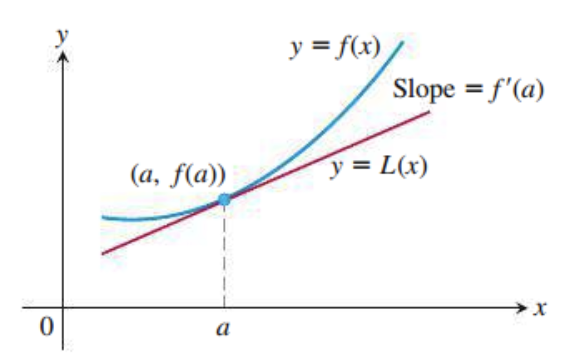
\includegraphics[width=3in]{img/linearization}
\end{center}
\begin{example}
Compute the linearization of $f(x)=\sqrt{1+x}$ at $x=0$.
\end{example}

\newpage

\begin{example}
Compute the linearization of $f(x)=\cos x$ at $x=\pi/2$.
\end{example}

\newpage

\begin{remark}\,
\begin{itemize}
\item The linearization of $y=f(x)$ at $x=a$ is most accurate when $x\approx a$.
\item In application, linearization is most often used to approximate changes (or errors) in $y$ corresponding to small changes (or errors) in $x$.
\item For this purpose, it is useful to make a change of variables $\dee x = x-a=\Delta x$.
\end{itemize}
\end{remark}
\begin{definition}\,
\begin{itemize}
\item The \textbf{independent differential} $\dee x = \Delta x$ represents a small change in $x$. 
\item The \textbf{dependent differential} $\dee y =\DS \frac{\dee y}{\dee x}\dee x$.
\end{itemize}
If $y=f(x)$, it is also common to write $\dee f = \dee y$.
\end{definition}
\begin{center}
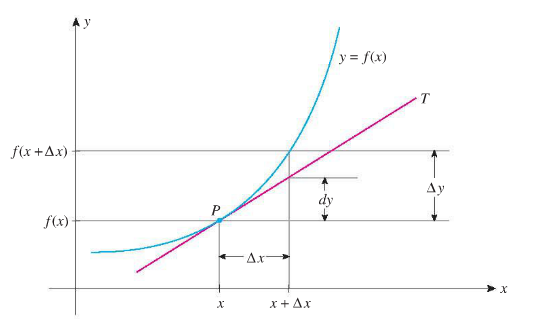
\includegraphics[width=3in]{img/differentials}
\end{center}
\begin{remark}\,
\begin{itemize}
\item If $\dee x$ is sufficiently small, then $\dee y\approx\Delta y$.
\item \underline{Caution}: When you write sloppy mathematics, you reinforce your belief in false and often ridiculous statements.
\begin{itemize}
\item The \underline{differential} $\dee x = \Delta x$ is a small change/error in $x$, and so has units of $x$.
\item The \underline{derivative} $\DS\frac{\dee y}{\dee x}$ is the rate of change of $y$ with respect to $x$, and so has units of $y$ per units of $x$.
\item The \underline{differential} $\dee y = \DS\frac{\dee y}{\dee x}\dee x$ is a approximate change/error in $y$, and so has units of $y$.
\end{itemize}
\item Be careful what you write: $\dee y\ne \DS\frac{\dee y}{\dee x}$.
\end{itemize}
\end{remark}

\newpage

\begin{example}
Compute $\dee y$ if $y=x^5+37x$.
Then compute its value when $x=1$ and $\dee x=0.2$.
\end{example}
\vfill

\begin{example}
Use differentials to estimate $\sqrt[3]{7.97}$.
\end{example}
\vfill

\newpage


\begin{remark}\,
\begin{itemize}
\item Differentials are often used to estimate the propagated error in a calculated quantity $y=f(x)$ given some bound on measured error $\Delta x = \dee x$.
\item Since we don't know $\dee x$ exactly but can usually assume that it is small, it is reasonable to use the approximation $\Delta y\approx \dee y$ for the propagated error in $y$.
\begin{center}
\begin{tabular}{c||cc}
error type & exact value & estimated value\\
\hline\hline
\textbf{absolute error} & $|\Delta y|$ & $|\dee y|$\\

\textbf{relative error} & $\left|\frac{\Delta y}{y}\right|$ & $\left|\frac{\dee y}{y}\right|$
\end{tabular}
\end{center}
\item \textbf{Percentage error} is just relative error expressed as a percentage.
\end{itemize}
\end{remark}

\begin{example}
Suppose you want to calculate the depth of a well by dropping a stone and timing how long it takes before you hear a splash.
How deep is the well if you hear a splash $t=5$ seconds after releasing the stone?
Use differentials to estimate how sensitive the calculation is to a 0.1 second error in measuring the time.  
\end{example}

\newpage

\begin{example}
Estimate the allowable percentage error in measuring the diameter $d$ of a sphere if the volume $V=\frac{4}{3}\pi r^3$ is to be calculated to within $3\%$.
\end{example}
